\ffigbox[\FBwidth]{%
\label{Fig:td1ex1c1}
}{
    \fbox{
        \begin{tikzpicture}[scale=1, every node/.style={circle, draw, fill=blue!20, inner sep=1pt, font=\scriptsize, minimum size=4mm}]
            \node (x1) at (0,0) {\(X_1\)};
            \node (x2) at (2,0) {\(X_2\)};
            \node (x3) at (4,0) {\(X_3\)};


            \node at (0,-1) {\(\scriptstyle 0\)};
            \node at (0,-2) {\(\scriptstyle 1\)};

            \node at (2,-1) {\(\scriptstyle 0\)};
            \node at (2,-2) {\(\scriptstyle 1\)};

            \node at (4,-1) {\(\scriptstyle 0\)};
            \node at (4,-2) {\(\scriptstyle 1\)};
            \node at (4,-3) {\(\scriptstyle 2\)};

            \draw (x1) -- (x2) node[midway, above] {\(\overset{4}{<}\)};
            \draw (x2) -- (x3) node[midway, above] {\(\overset{4}{<}\)};
            
        \end{tikzpicture}
    }
}